\documentclass[letterpaper]{article} 
\usepackage[utf8]{inputenc}
\usepackage[T1]{fontenc}
\usepackage{amsmath}
\usepackage{amsfonts}
\usepackage{amssymb}
\usepackage{hyperref}
\usepackage[version=4]{mhchem}
\usepackage{stmaryrd}
\usepackage[dvipsnames]{xcolor}
\colorlet{LightRubineRed}{RubineRed!70}
\colorlet{Mycolor1}{green!10!orange}
\definecolor{Mycolor2}{HTML}{00F9DE}
\usepackage{graphicx}
\usepackage{amsmath}
\usepackage{graphicx}
\usepackage{capt-of}
\usepackage{lipsum}
\usepackage{fancyvrb}
\usepackage{tabularx}
\usepackage{listings}
\usepackage[export]{adjustbox}
\graphicspath{ {./images/} }
\usepackage[utf8]{inputenc}
\usepackage[english]{babel}
\usepackage{float}
\usepackage{lipsum}
\usepackage{graphicx}
\usepackage{float}
\usepackage[margin=0.7in]{geometry}
\usepackage{amsmath}
\usepackage{graphicx}
\usepackage{capt-of}
\usepackage{tcolorbox}
\usepackage{lipsum}
\usepackage{graphicx}
\usepackage{float}
\usepackage{listings}
\usepackage{hyperref} 
\usepackage{xcolor} % For custom colors
\lstset{
	language=Python,                % Choose the language (e.g., Python, C, R)
	basicstyle=\ttfamily\small, % Font size and type
	keywordstyle=\color{blue},  % Keywords color
	commentstyle=\color{gray},  % Comments color
	stringstyle=\color{red},    % String color
	numbers=left,               % Line numbers
	numberstyle=\tiny\color{gray}, % Line number style
	stepnumber=1,               % Numbering step
	breaklines=true,            % Auto line break
	backgroundcolor=\color{black!5}, % Light gray background
	frame=single,               % Frame around the code
}
\usepackage{float}
\usepackage[]{amsthm} %lets us use \begin{proof}
	\usepackage[]{amssymb} %gives us the character \varnothing
	

	
	\title{Homework Midterm, MATH 5010}
	\author{Zongyi Liu}
	\date{Mon, Feb 17, 2025}
	\begin{document}
		\maketitle
		
\section{Question 1}
\subsection{Solve it Using Matlab}
		Matlab option model. Download from Courseworks matlab option model files \texttt{BlackScholesStocks.m} and \\ \texttt{BlackScholesGraph.m} and put them in the same directory. \texttt{BlackScholesStocks.m} contains the function that calculates the Black Scholes price for options on non-dividend paying stocks. \texttt{BlackScholesGraph.m} is a script that makes a graph of option price as a function of stock price. Type at Matlab prompt \texttt{>BlackScholesGraph} and the script will be executed, and the graph will appear. Now modify the file \texttt{BlackScholesStocks.m} so that the function now calculates the price of options on stocks paying continuous dividends at a rate q. Modify the file \texttt{BlackScholesGraph.m} so that it now plots graph of a call with the same parameters as before but with the dividend yield $\mathrm{q}=2 \%$ and the new strike price 11. Submit printouts of code and graph.

		\textbf{Answer}
		The modified \texttt{BlackScholesStocks.m} file is:
		
		\begin{lstlisting}
     function Price = BlackScholesStocks(callput, S, K, r, q, sigma, T)
     
     % Adjusted d1 and d2 formulas with continuous dividend yield q
     d1 = (log(S/K) + (r - q + 0.5 * sigma^2) * T) / (sigma * sqrt(T));
     d2 = d1 - sigma * sqrt(T);
     
     % Define normcdf alternative using erf
     function N = norm_cdf_approx(x)
     N = 0.5 * (1 + erf(x / sqrt(2)));
     end
     
     if callput == 'c'   
     % for call with dividends
     N1 = norm_cdf_approx(d1);
     N2 = norm_cdf_approx(d2);
     Price = S * exp(-q * T) * N1 - K * exp(-r * T) * N2;
     
     elseif callput == 'p'
     % for put with dividends
     N1 = norm_cdf_approx(-d1);
     N2 = norm_cdf_approx(-d2);
     Price = K * exp(-r * T) * N2 - S * exp(-q * T) * N1;
     
     else
     error('Invalid option type. Use ''c'' for call or ''p'' for put.');
     end
     end
     
		\end{lstlisting}
	
	And the modified \texttt{BlackScholesGraph.m} file is:
	
	\begin{lstlisting}
     clear all;
     clc;
     
     % Parameters
     dx = 0.1; 
     maxX = 20; 
     X = dx:dx:maxX; 
     Strike = 11; % Updated strike price
     Rate = 0.01;
     Time = 1;
     Volatility = 0.3;
     DividendYield = 0.02; % q = 2%
     
     Y = max(X - Strike, 0); % Call payoff at expiration
     
     % Preallocate Z
     Z = zeros(1, length(X));
     
     % Compute option price with dividends
     i = 0;
     for xVal = X  % Using xVal instead of X to avoid variable conflict
     i = i + 1;
     Z(i) = BlackScholesStocks('c', xVal, Strike, Rate, DividendYield, Volatility, Time);
     end
     
     % Plot
     plot(X, Z, X, Y);
     xlabel('Stock Price');
     ylabel('Option Value');
     legend('Black-Scholes Call Price', 'Payoff at Expiration');
     grid on;
	\end{lstlisting}
		
		The print-out will be:
		
		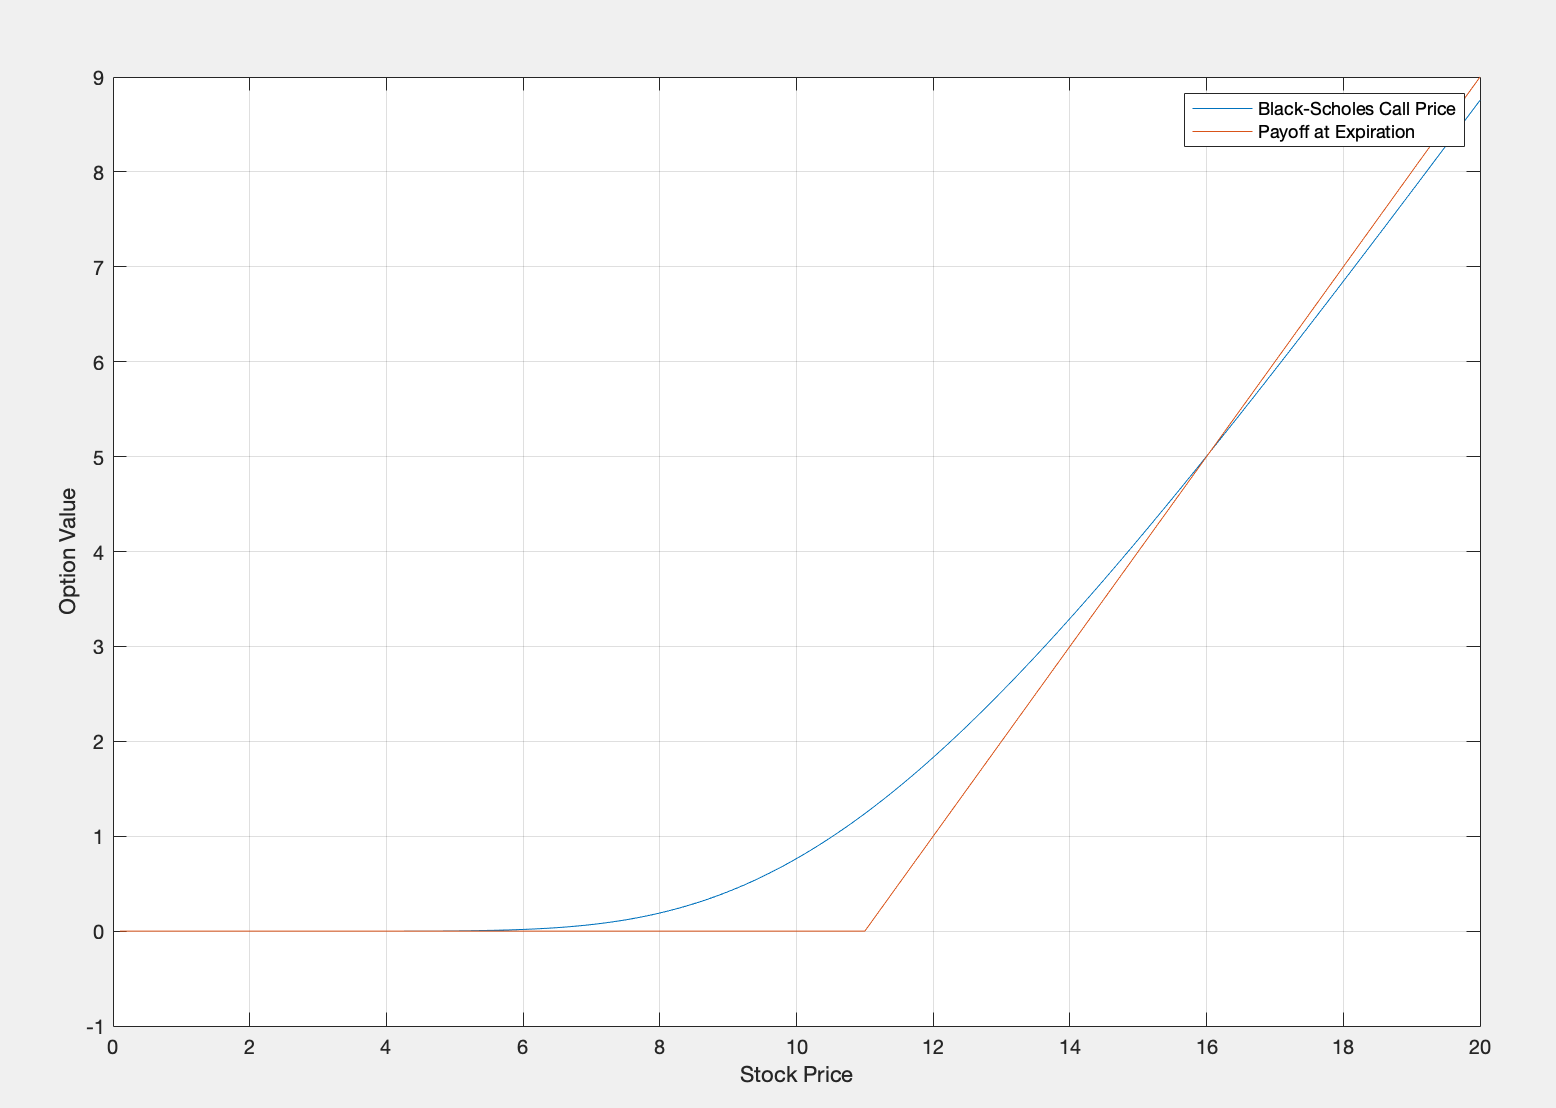
\includegraphics[max width=\textwidth, center]{Q1}
		\captionof{figure}{Black-Scholes Call}
		\pagebreak
		\subsection{Solve it Using R}
		I also tried to solve it using R.
		
		\begin{lstlisting}
     # Parameters
     dx <- 0.1
     maxX <- 20
     X <- seq(dx, maxX, by=dx)  # Stock price range
     Strike <- 11  # Updated strike price
     Rate <- 0.01  # Risk-free rate
     Time <- 1  # Time to maturity
     Volatility <- 0.3  # Volatility
     DividendYield <- 0.02  # Dividend yield
     
     # Black-Scholes formula for call option price
     d1 <- function(S) {
     	(log(S / Strike) + (Rate - DividendYield + 0.5 * Volatility^2) * Time) / (Volatility * sqrt(Time))
     }
     d2 <- function(S) {
     	d1(S) - Volatility * sqrt(Time)
     }
     CallPrice <- function(S) {
     	S * exp(-DividendYield * Time) * pnorm(d1(S)) - Strike * exp(-Rate * Time) * pnorm(d2(S))
     }
     
     # Payoff at expiration (European call option payoff)
     Payoff <- function(S) {
     	pmax(S - Strike, 0)
     }
     
     # Calculate stock price and corresponding call option price and payoff
     callOptionPrice <- CallPrice(X)
     payoffAtExpiration <- Payoff(X)
     
     # Plotting both the Black-Scholes Call Price and Payoff at Expiration
     plot(X, callOptionPrice, type="l", col="blue", lwd=2, 
     xlab="Stock Price", ylab="Option Value",
     ylim=c(0, max(c(callOptionPrice, payoffAtExpiration))))
     lines(X, payoffAtExpiration, col="red", lwd=2)
     legend("topleft", legend=c("Black-Scholes Call Price", "Payoff at Expiration"),
     col=c("blue", "red"), lwd=c(2, 2))
     grid()
		\end{lstlisting}
	
	And the printout is as below:
	
		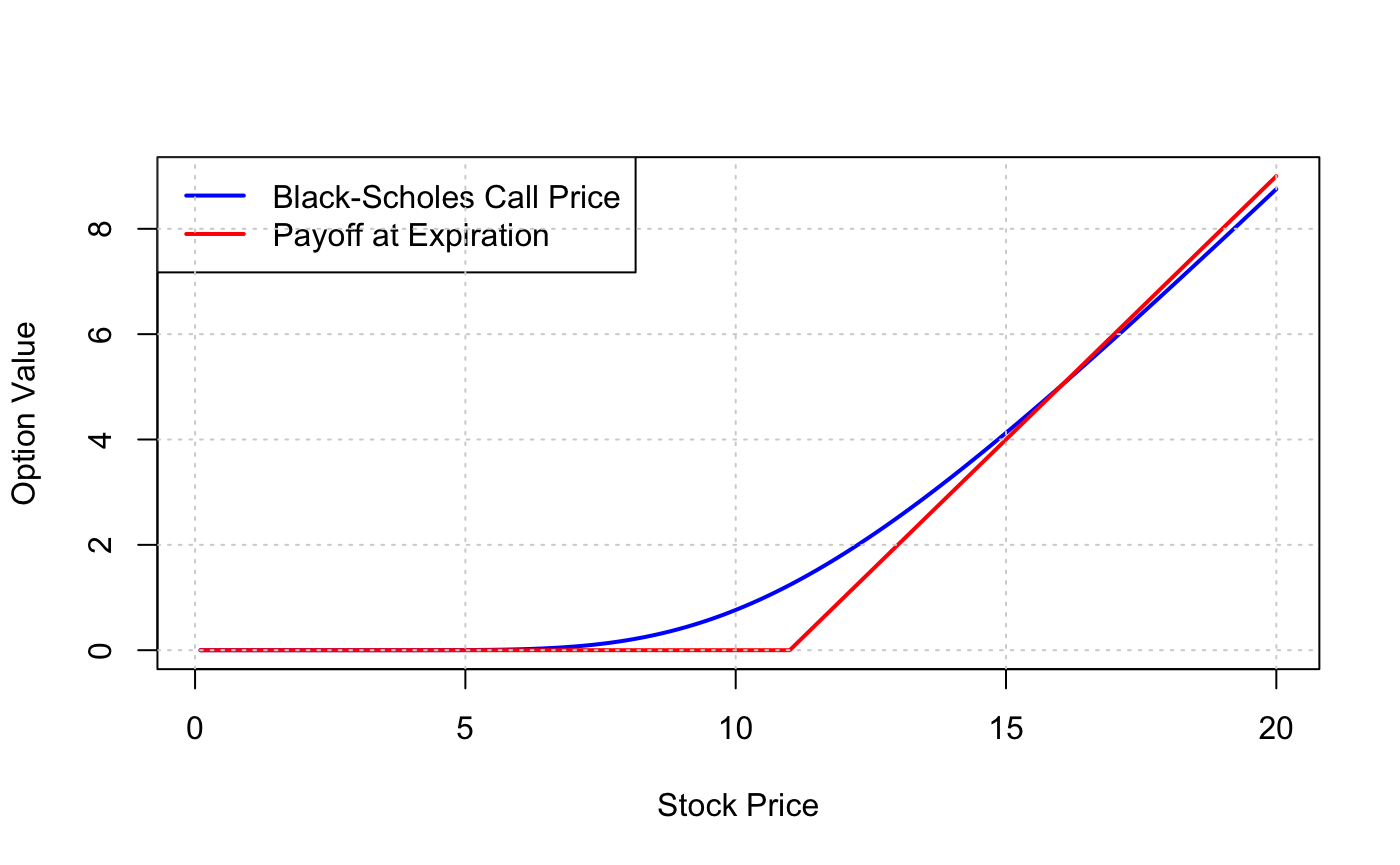
\includegraphics[max width=\textwidth, center]{Q1_2}
		\captionof{figure}{Black-Scholes Call}
		\pagebreak
		
		\section{Question 2}
		Download matlab Brownian motion model from the courseworks. Modify it to Geometric Brownian motion with starting value $\mathrm{X_0}=100$, growth rate $\mu=0.14$, volatility $\sigma=0.28$ and 5000 trajectories. Check that the code works. Try out 50,000 trajectories. Try out 100,000 trajectories. Submit the code printout and the graph printout for 5000 trajectories.
		
		\textbf{Answer}
		\subsection{Solve it Using Matlab}
		
		The modified code will be:
		
		\begin{lstlisting}
     % Parameters
     M = 100000;   % Number of trajectories
     N = 250;    % Number of steps in each trajectory
     X0 = 100;   % Initial value
     T = 1;      % Final time (years)
     mu = 0.14;  % Growth rate (drift)
     sigma = 0.28; % Volatility
     
     dt = T / N;         % Time step
     Sqrtdt = sqrt(dt);  % Square root of time step
     
     % Preallocate matrix for efficiency
     X = zeros(M, N + 1);
     X(:, 1) = X0; % Set initial value for all trajectories
     
     % Generate M trajectories
     for j = 1:M
     for i = 2:N+1
     dW = randn(1,1) * Sqrtdt; % Brownian increment
     X(j, i) = X(j, i-1) * exp((mu - 0.5 * sigma^2) * dt + sigma * dW);
     end
     end
     
     % Time vector
     t = linspace(0, T, N + 1);
     
     % Plot multiple trajectories
     figure;
     plot(t, X');
     xlabel('Time (years)');
     ylabel('Stock Price');
     grid on; \end{lstlisting}
 
		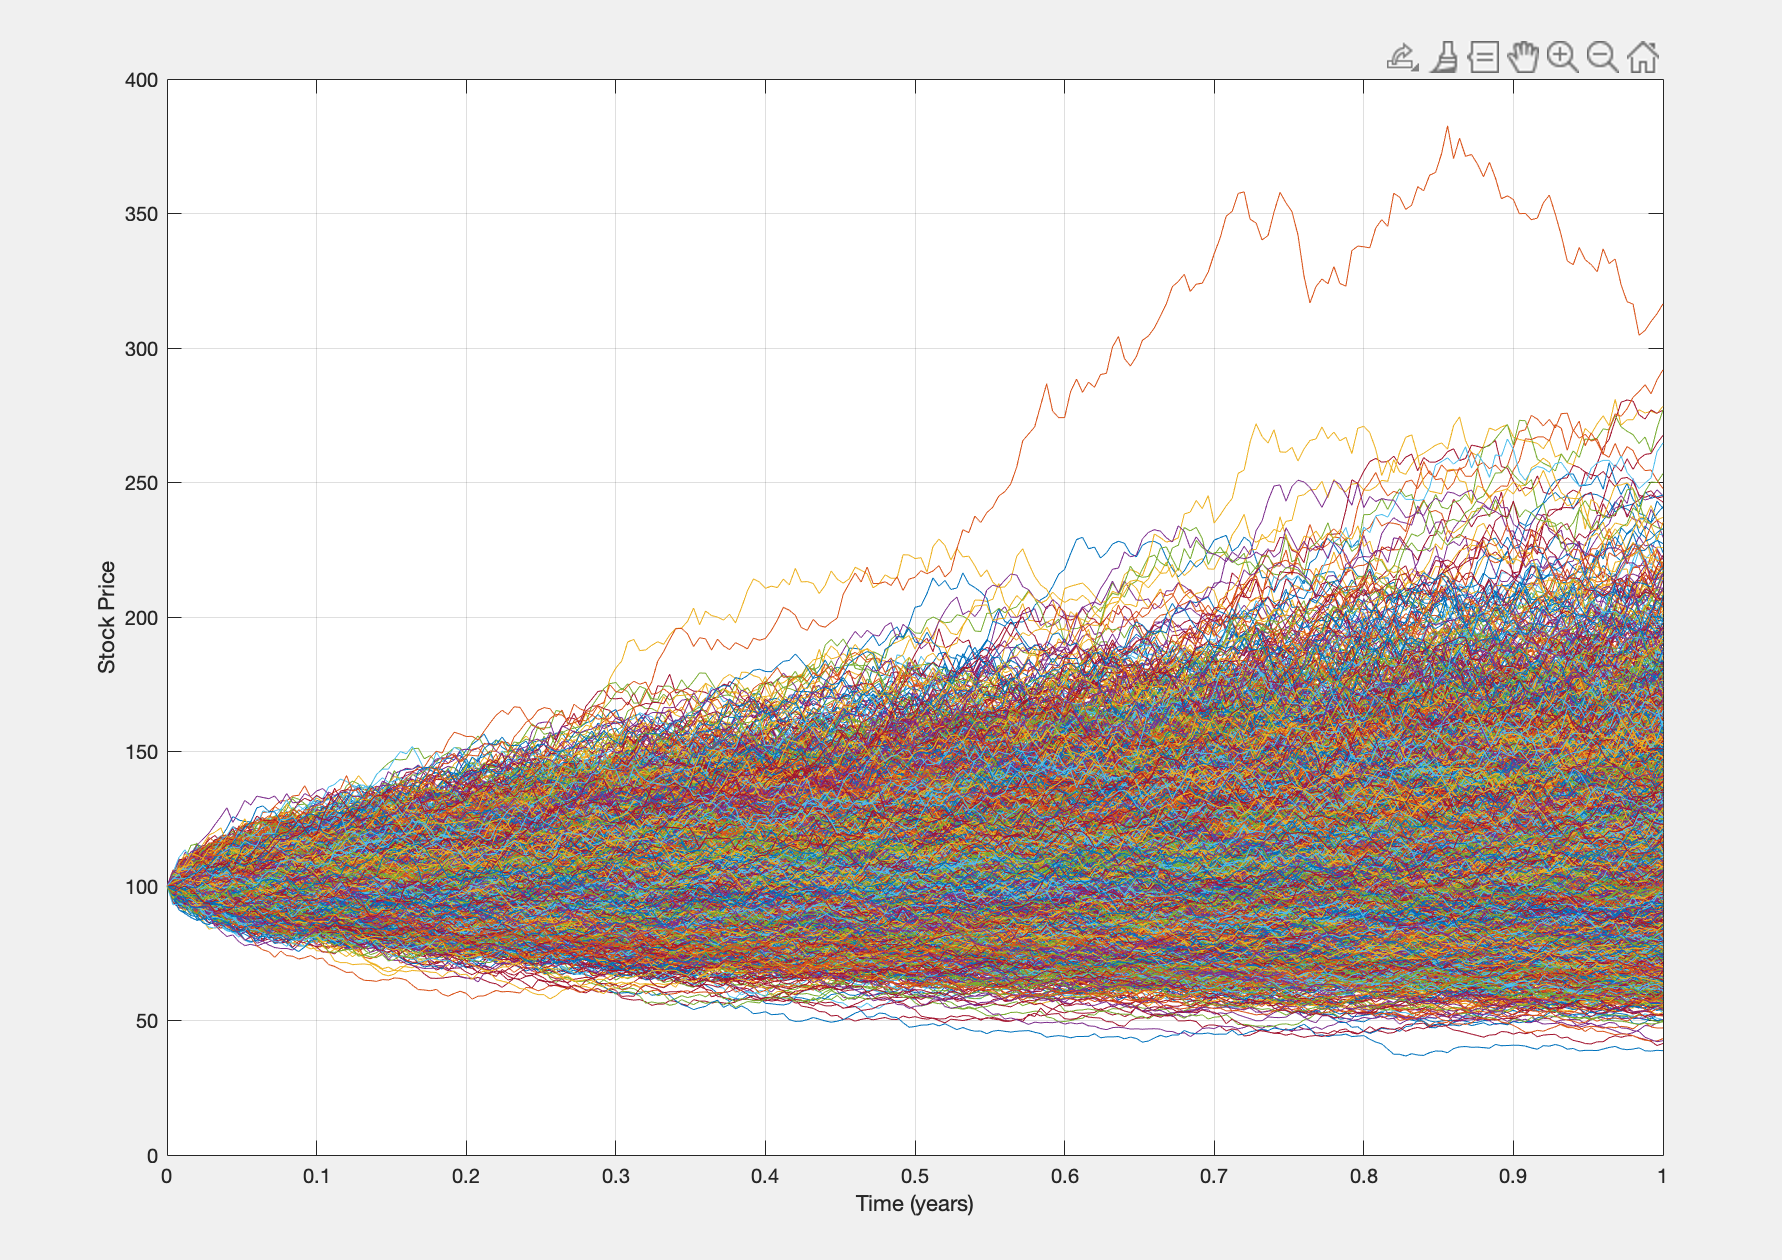
\includegraphics[max width=\textwidth, center]{Q2_5000}
		\captionof{figure}{Geometric Brownian Motion with 5,000 Trajectories in MATLAB}
		
		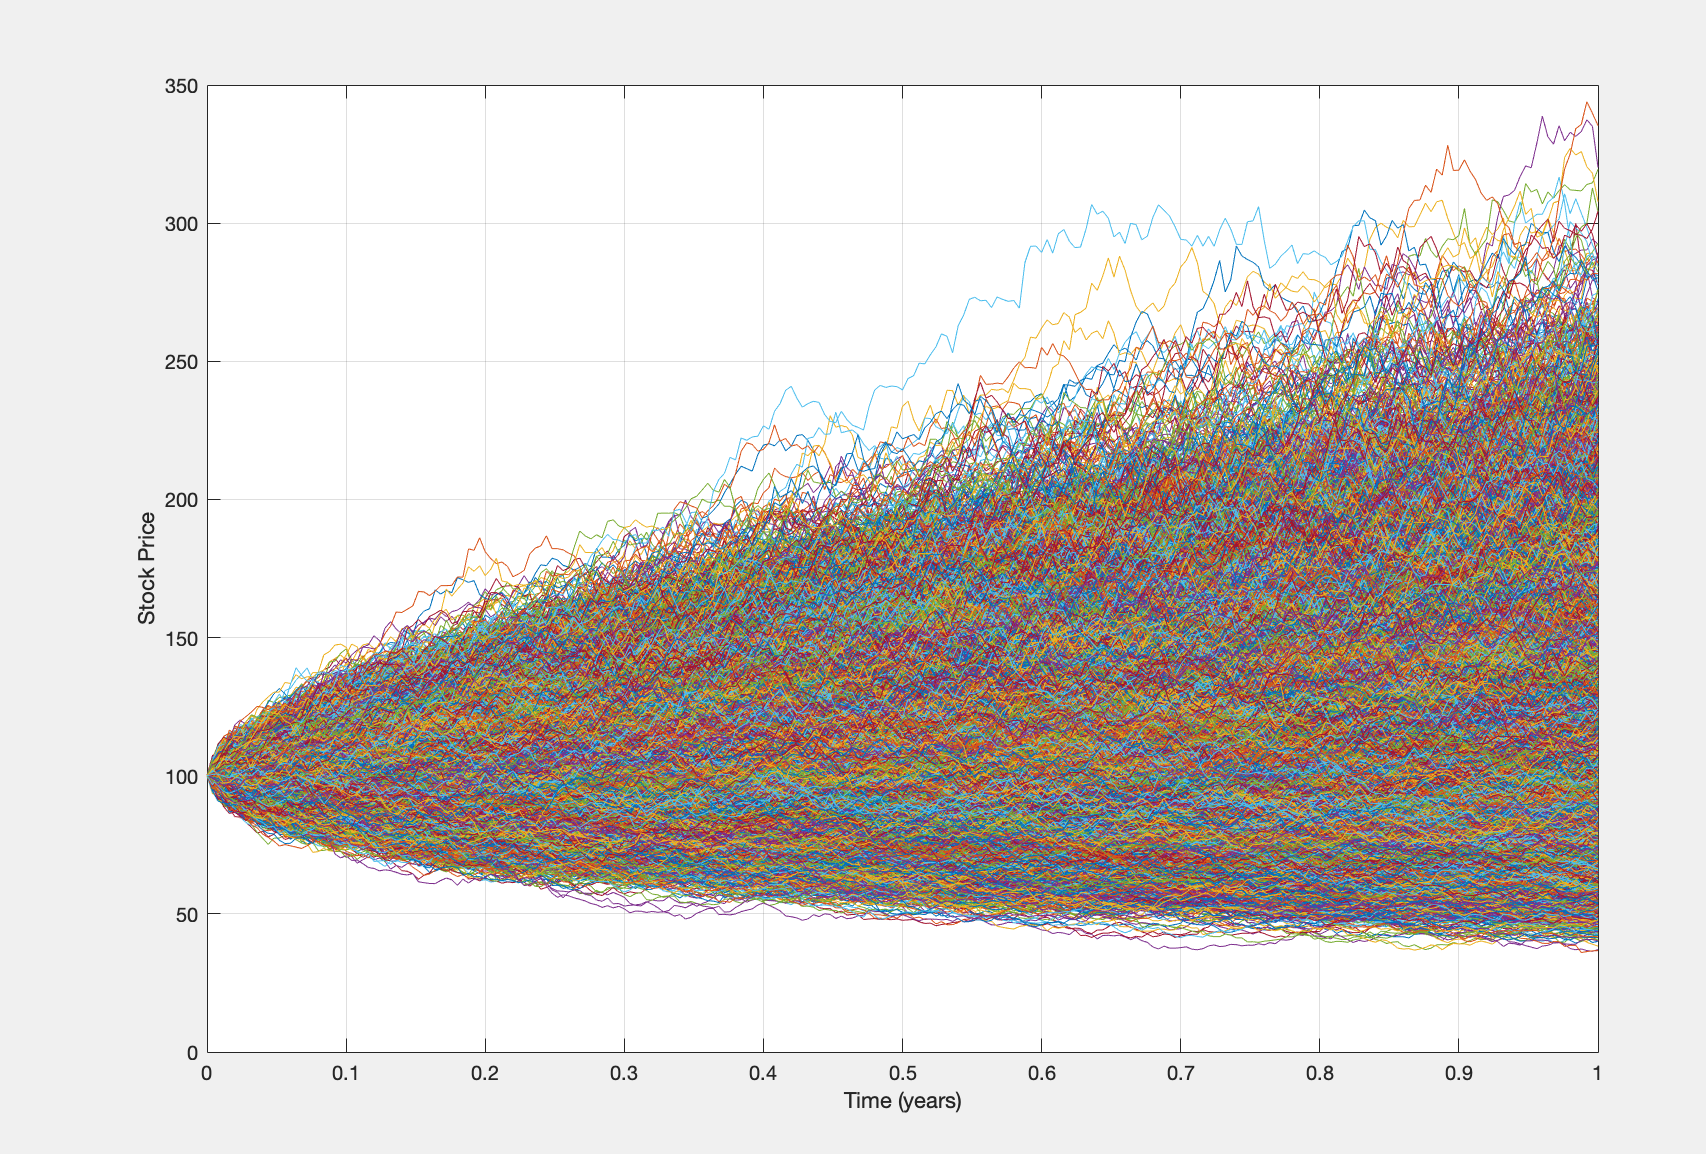
\includegraphics[max width=\textwidth, center]{Q2_50000}
		\captionof{figure}{Geometric Brownian Motion with 50,000 Trajectories in MATLAB}
		
		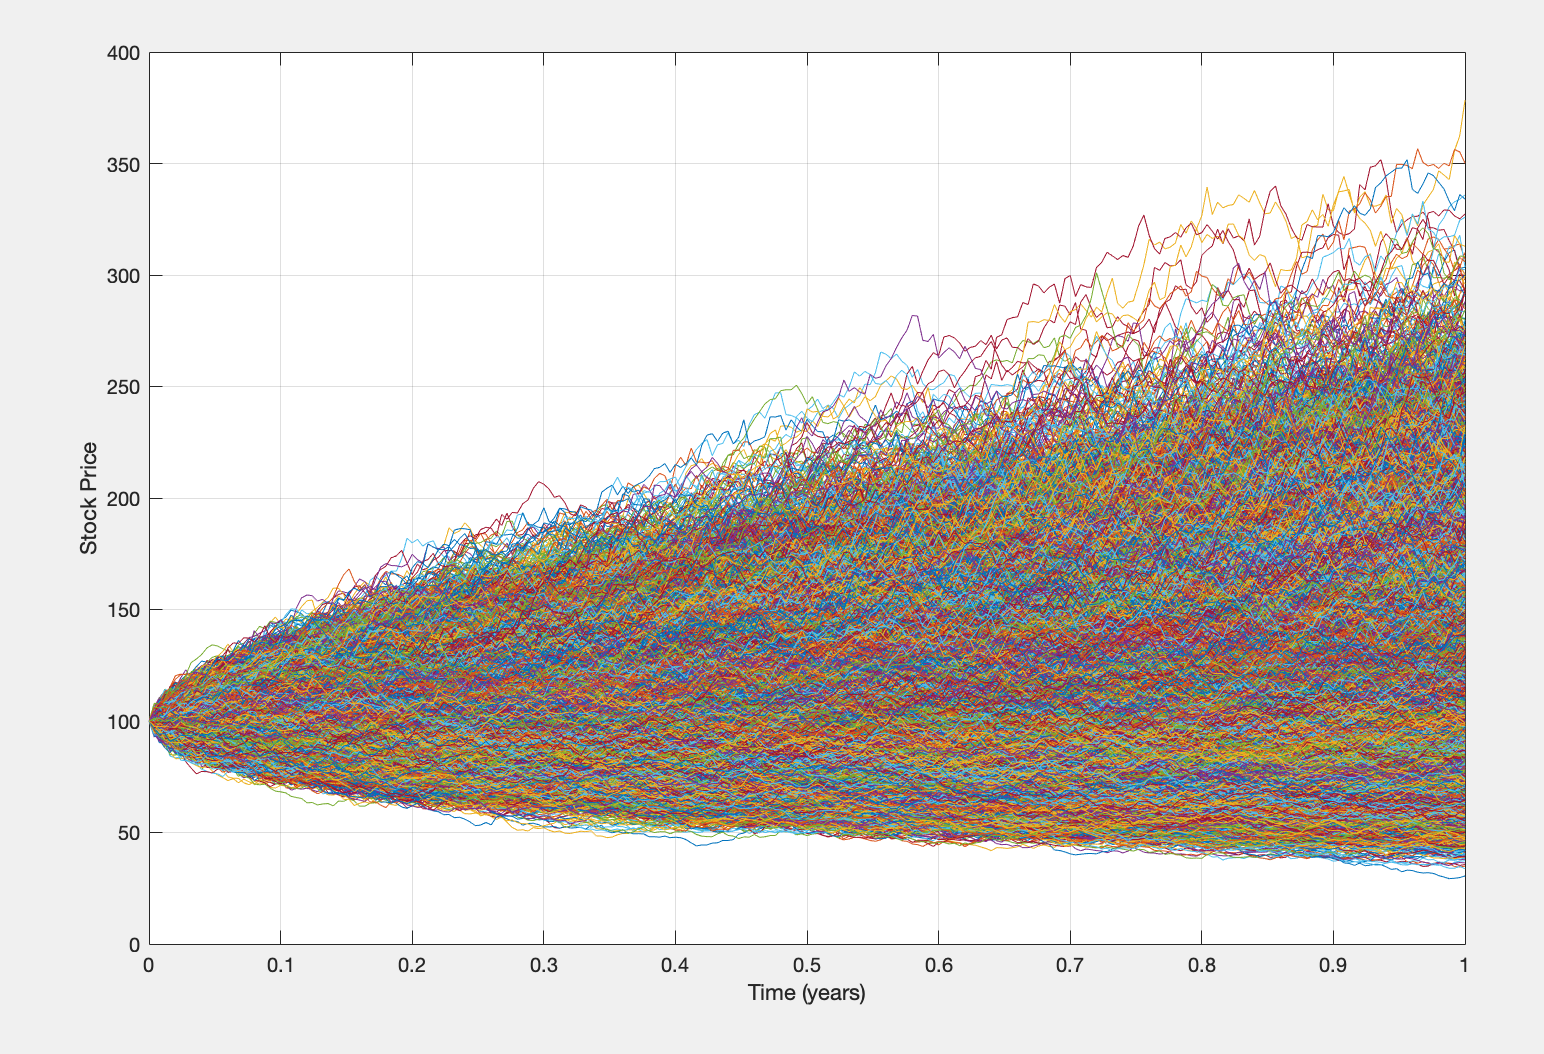
\includegraphics[max width=\textwidth, center]{Q2_100000}
		\captionof{figure}{Geometric Brownian Motion with 100,000 Trajectories in MATLAB}
		
		
		\subsection{Solve it Using R}
			 
		 I also did it in R, and the codes are as below:
			 
			 \begin{lstlisting}
     library(ggplot2)
     library(tidyr)
     
     # Parameters
     X0 <- 1000
     mu <- 0.14
     sigma <- 0.20
     n <- 50000    # Number of paths
     T <- 1      # Time horizon
     N <- 250    # Number of time steps
     dt <- T / N # Time increment
     
     # Generate time vector
     time <- seq(0, T, by = dt)
     
     # Initialize matrix to store trajectories
     X <- matrix(NA, nrow = N + 1, ncol = n)
     X[1, ] <- X0
     
     # Simulate GBM
     set.seed(123)  # For reproducibility
     for (i in 1:n) {
     	for (j in 2:(N + 1)) {
     		dW <- rnorm(1, mean = 0, sd = sqrt(dt))
     		X[j, i] <- X[j - 1, i] * exp((mu - 0.5 * sigma^2) * dt + sigma * dW)
     	}
     }
     
     # Convert matrix to data frame for ggplot
     X_df <- as.data.frame(X)
     X_df$time <- time
     
     # Reshape data from wide to long format using tidyr's pivot_longer
     X_long <- X_df %>%
     pivot_longer(cols = -time, names_to = "trajectory", values_to = "price")
     
     # Plot the trajectories with different colors
     ggplot(X_long, aes(x = time, y = price, color = trajectory)) +
     geom_line(alpha = 0.7) +  # Set transparency for better visibility
     labs(
     x = "Time",
     y = "Price",
     ) +
     theme_minimal() +
     scale_color_viridis_d()+  # Use a perceptually uniform color palette
     theme(legend.position = "none")  # Remove the legend
			 \end{lstlisting}
			
			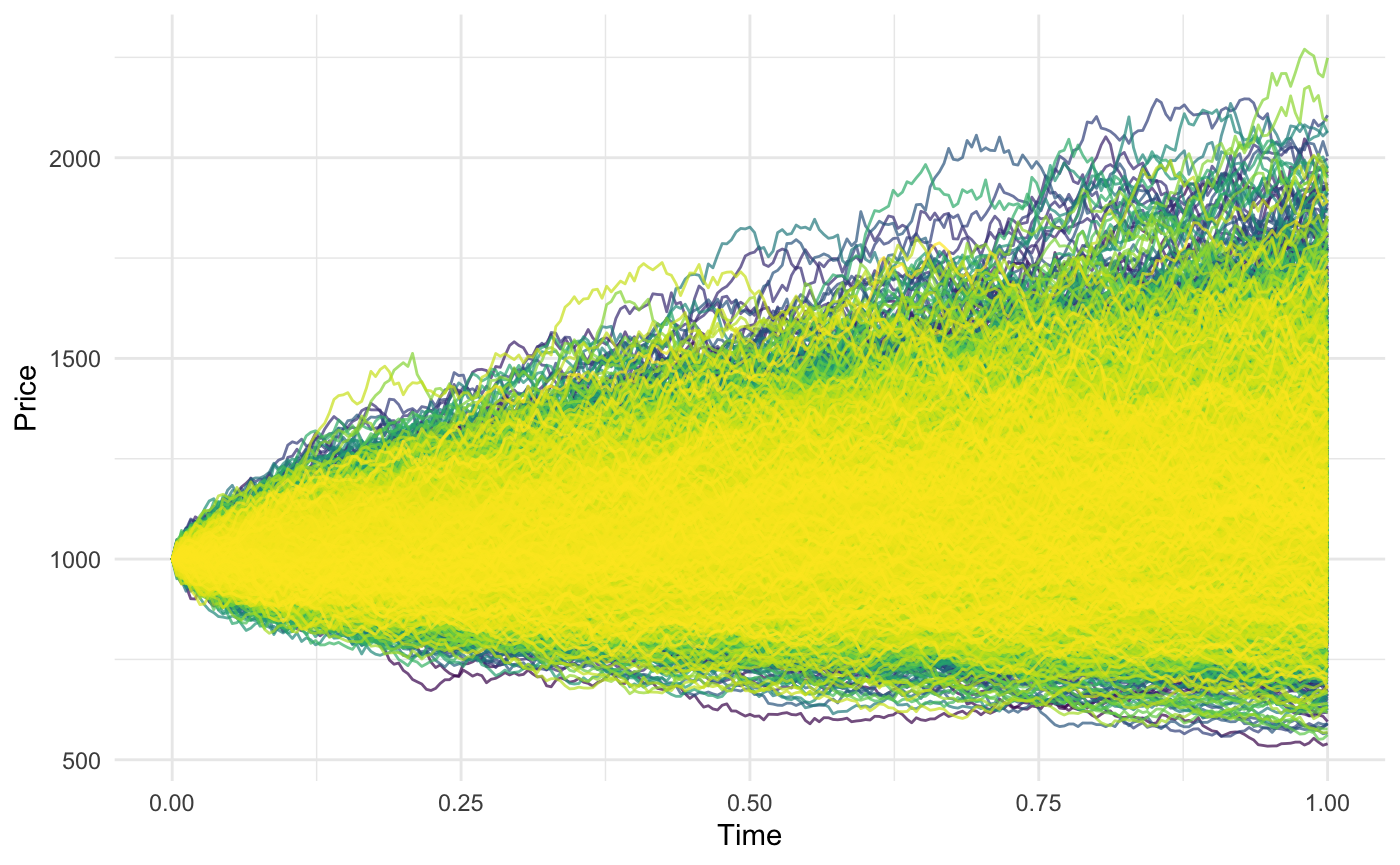
\includegraphics[max width=\textwidth, center]{Q2_R_5000}
			\captionof{figure}{Geometric Brownian Motion with 5,000 Trajectories in R}
			
			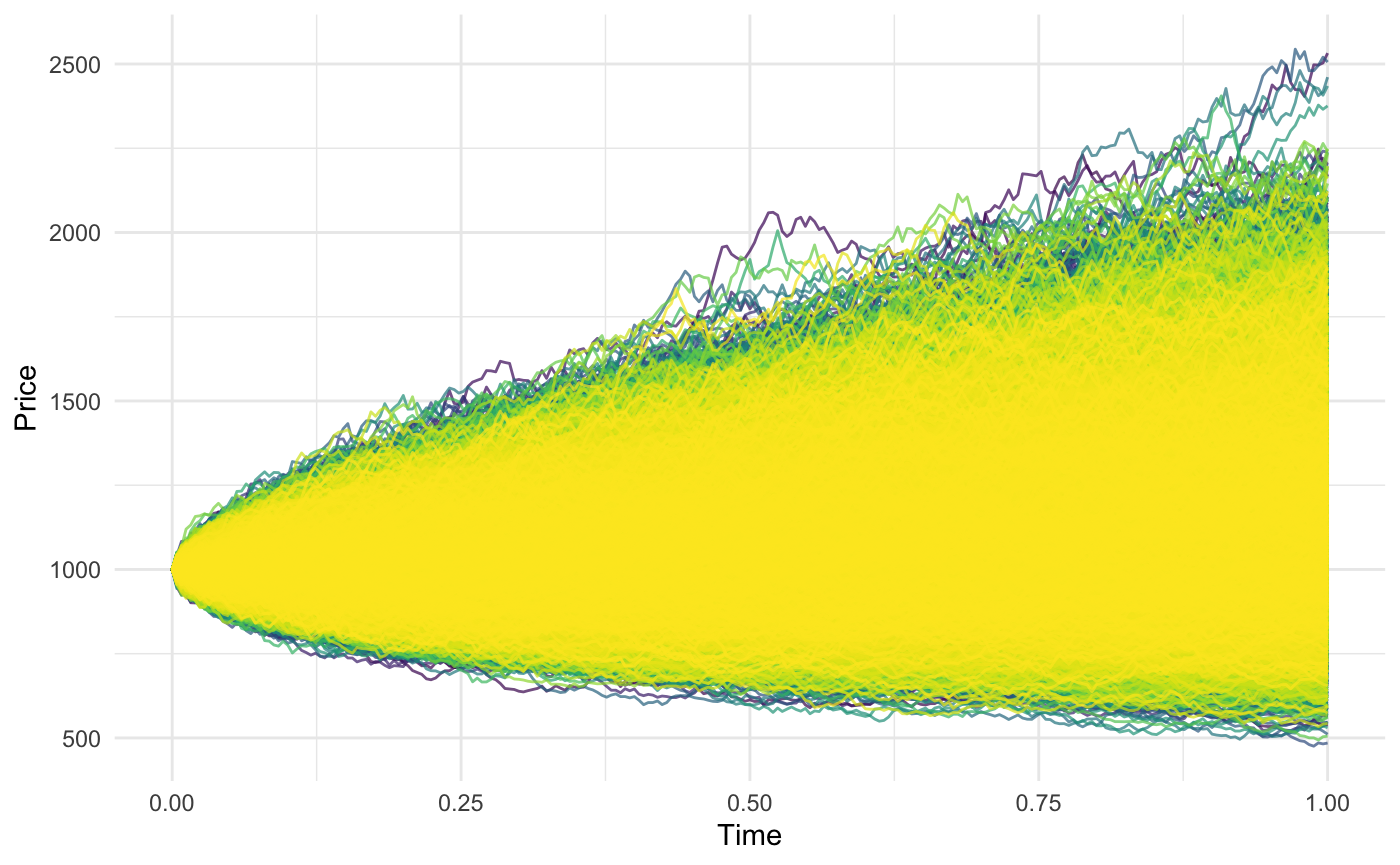
\includegraphics[max width=\textwidth, center]{Q2_R_50000}
			\captionof{figure}{Geometric Brownian Motion with 50,000 Trajectories in R}
		\pagebreak
		
		\section{Question 3}
		Using arbitrage arguments explain why the price of an American call option on a stock paying no dividends should be the same as the price of a corresponding European call. Why American calls on a non-dividend paying stock should not be exercised early.
		
		\textbf{Answer}
		
		For an American call option on a non-dividend-paying stock, the price should be the same as the corresponding European call option. We can show this using an arbitrage argument.
		
		Let $C_E$ be the price of a {European call} and $C_A$ be the price of a {American call} with the same strike price and maturity. Since an American call option has at least the same flexibility as a European call, we must have that $C_A \geq C_E$. 
		
		Now, suppose $C_A > C_E$. An arbitrageur could execute the following strategy:
		
		\begin{itemize}
			\item Sell the American call at a higher price $C_A$.
			\item Buy the European call at a lower price $C_E$.
			\item Since both options have the same payoff at expiration, this results in a risk-free profit.
		\end{itemize}
		
		Since arbitrage opportunities cannot exist in an efficient market, we conclude that:
		$$
			C_A = C_E
		$$
		
		for an American call on a \underline{non-dividend-paying stock}.
		
		For this kind of settings, early exercise is never optimal due to the following three reasons:
		
		\begin{itemize}
		
		\item The first is that there are no additional cash flow before expiration. When an option holder exercises early, they pay $K$ (the strike price) and receive the stock worth $S_t$. However, the holder loses the \underline{time value} of the option (Hull, Ch. 10.5, pg 225, 8th Edition). Instead of exercising, they could sell the option at a higher price in the market. we can see this mathematically:
		
		$$
		\begin{aligned}
		E: &\text{one American call}c, X e^{-r(T-t)}\text{cash}\\
		&F: \text{one share} S.
	\end{aligned}
$$

		If the exercise time is $\tau<T$, the value of $E$ is
		$$
		\begin{aligned}
			E & =(S-X)+X e^{-r(T-t)} \\
			& <S=F
		\end{aligned}
		$$
		
		If the exercise is at $t=T$, then
		$$
		\begin{aligned}
			E & =\max (S-X, 0)+X \\
			& =\max (S, X) \\
			& \geq S=F
		\end{aligned}
		$$
		
		It follows that $E \geq F$ for all times, so that one should never take $t<T$.
		
		\item The second reason is that holding the call option means postponing the payment of $K$. Since money has time value, it is better to delay payment as long as possible. Exercising early forces the holder to pay $K$ sooner, which is suboptimal.
		
		\item And the last reason is that stock price can increase further. If the option is exercised early, the holder locks in an immediate profit of $S_t - K$. However, if the option is held longer, the stock price could increase further, making the option even more valuable. In Hull's book, he argues: "relates to the insurance that it provides. A call option, when held instead of the stock itself, in effect insures the holder against the stock price falling below the strike price. Once the option has been exercised and the strike price has been exchanged for the stock price, this insurance vanishes." (Ch.10.5, pg 226, 8th Edition) So we can say that early exercise \underline{limits the upside potential and cut the insurance}.
		
	\end{itemize}
		Since early exercise never benefits the holder of an American call on a non-dividend-paying stock, its price must be the same as the corresponding European call. American call holders should \underline{never exercise early} because holding the option provides greater flexibility and potential value than exercising and holding the stock.
		
		Thus, we conclude that $C_A = C_E$, for an American call on a {non-dividend-paying stock}, and {early exercise is never optimal}.

		
		\pagebreak
		
		\section{Question 4}
		Why when the stock pays dividends the argument of the problem 3 can not be used. Give a numerical example (choosing ${x},\ {k},\ {r},\ {T}-{t}, \sigma$) in which it is obvious (without any formulas) that American put price on a nondividend paying stock is larger than the corresponding European put price.
		
		\textbf{Answer}
		\subsection{Dividends-Paying Scenario}
		When there are dividends, the arugement in Problem 3 is not valid,  its price typically drops by the amount of the dividend on the ex-dividend date. For call options, a lower stock price reduces the option's value. For American call options, the holder has the right to exercise the option at any time before expiration. If a dividend is paid, the holder may choose to exercise the option early to capture the stock's value before the price drops due to the dividend. whereas for European call options, the holder can only exercise the option at expiration. They cannot avoid the stock price drop caused by the dividend payment.
		
		 If we expand further, when dividends are paid, mostly it can only be optimal to exercise at a time immediately before the stock goes ex-dividend for an American call option (Hull, Ch. 14.12, pg 320, 8th Edition, and the mathematical demonstrations are derived from this chapter). Assuming that $n$ ex-dividend dates are anticipated and that they are at times $t_1, t_2, \ldots, t_n$, with $t_1<t_2<\cdots<t_n$. The dividends corresponding to these times will be denoted by $D_1, D_2, \ldots, D_n$.
		
		We can start by considering the possibility of early exercise just prior to the final ex-dividend date (i.e., at time $t_n$ ). If the option is exercised at time $t_n$, the investor receives$
		S\left(t_n\right)-K$
		
		Here $S(t)$ denotes the stock price at time $t$. If the option is not exercised, the stock price drops to $S\left(t_n\right)-D_n$. The value of the option is then greater than
		$$
		S\left(t_n\right)-D_n-K e^{-r\left(T-t_n\right)}
		$$
		
		It follows that, if
		$$
		S\left(t_n\right)-D_n-K e^{-r\left(T_n t_n\right)} \geqslant S\left(t_n\right)-K
		$$
		that is,
		$$
		D_n \leqslant K\left[1-e^{-r\left(T-t_n\right)}\right]
		$$
		it cannot be optimal to exercise at time $t_n$. On the other hand, if $
		D_n>K\left[1-e^{-n\left(T-t_n\right)}\right]$
		
		for any reasonable assumption about the stochastic process followed by the stock price, it can be shown that it is always optimal to exercise at time $t_n$ for a sufficiently high value of $S\left(t_n\right)$. The inequality in equation above will tend to be satisfied when the final e: dividend date is fairly close to the maturity of the option (i.e., $T-t_n$ is small) and th dividend is large.
		
		For the next time $t_{n-1}$, the penultimate ex-dividend date. If the option is exercise immediately prior to time $t_{n-1}$, the investor receives $S\left(t_{n-1}\right)-K$. If the option is $n$, exercised at time $t_{n-1}$, the stock price drops to $S\left(t_{n-1}\right)-D_{n-1}$ and the carlie subsequent time at which exercise could take place is $t_n$.  A lower bound to the option price if it is not exercised at time $t_{n-1}$ is:
		$$
		S\left(t_{n-1}\right)-D_{n-1}-K e^{-r\left(t_n-t_{n-1}\right)}
		$$
	
	If
		$$
		S\left(t_{n-1}\right)-D_{n-1}-K e^{-\left(\left(t_n-t_{n-1}\right)\right.} \geqslant S\left(t_{n-1}\right)-K
		$$
		or
		$$
		D_{n-1} \leqslant K\left[1-e^{-\int\left(t_n-t_{n-1}\right)}\right]
		$$
		it is not optimal to exercise immediately prior to time $t_{n-1}$. Similarly, for any $i<n$,
		$$
		D_i \leqslant K\left[1-e^{-r\left(t_{i+1}-t_i\right)}\right]
		$$
		it is not optimal to exercise immediately prior to time $t_i$.
		The above inequality is approximately equivalent to:
		$$
		D_i \leqslant K r\left(t_{i+1}-t_i\right)
		$$
		
		Assuming that $K$ is fairly close to the current stock price, this inequality is satisfies when the dividend yield on the stock is less than the risk-free rate of interest, and this is usually the case. 
		
		We can conclude from the derivations above that in most of cases, doing an early exercise for American call option is optimal, thus it will not stay the same as the European call option as did in Problem 3, and it changes the argument. 
				
		\subsection{Put Option on Nondividend Paying Stock}
			
			
			We can get a simple numerical example to show that the {American put option} on a non-dividend-paying stock can be more valuable than the corresponding {European put option}. This happens because the American put option allows for \underline{early exercise}, which can be advantageous in certain scenarios.
			
			\begin{itemize}
				\item Stock price \( S = 100 \),
				\item Strike price \( K = 110 \),
				\item Risk-free rate \( r = 5\% \),
				\item Time to maturity \( T - t = 1 \) year,
				\item Volatility \( \sigma = 20\% \),
				\item Dividends: None.
			\end{itemize}
			
			
			Suppose during the life of the option, the stock price drops significantly (e.g., due to a market crash or bad news). Let’s say the stock price drops to \( S = 80 \) at some point before expiration.
			
		The holder of the American put option can \underline{exercise early} when the stock price is \( S = 80 \). The payoff from early exercise is $K - S = 110 - 80 = 30$. By exercising early, the holder locks in a profit of {30} and avoids the risk of the stock price recovering later.
			
		Whereas the holder of the European put option \underline{cannot exercise early} and must wait until expiration. If the stock price recovers to \( S = 90 \) by expiration, the payoff is $
				K - S = 110 - 90 = 20$. The European put option holder receives only {20}, which is less than the American put option holder’s payoff of {30}.
			
				We can say that the American put option allows the holder to {capture the maximum payoff} when the stock price drops significantly, even if the stock price later recovers. The European put option holder is {stuck waiting until expiration} and may miss the opportunity to lock in a higher payoff.
			

			
			Thus, it is clear that the {American put option is more valuable} than the European put option when the stock price drops significantly, even if the stock pays no dividends. This demonstrates the value of the \underline{early exercise feature} in American options.
			
			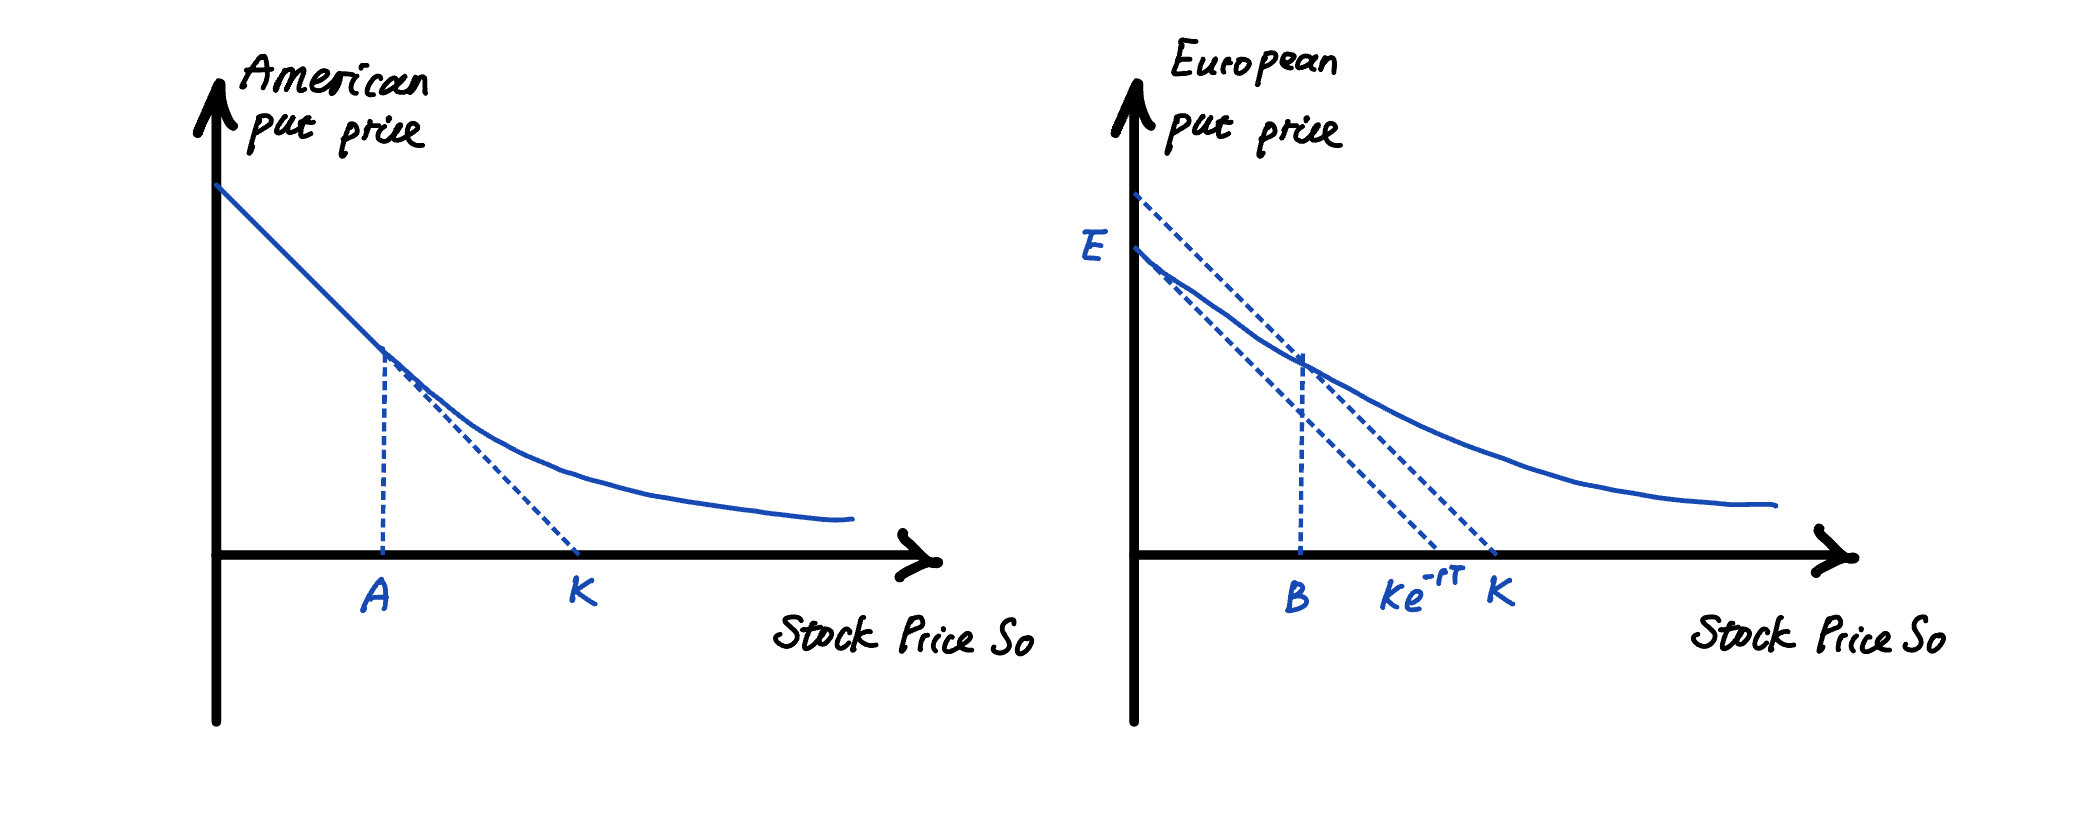
\includegraphics[max width=\textwidth, center]{Q4}
			\captionof{figure}{Comparison of American and European put Options with the Stock Price}
		
		\pagebreak
		
		\section{Question 5}
		\subsection{Part a}
		
		The stock price is 40 the volatility of the stock is $20 \%$. Assuming that the time to expiration is 3 months and the interest rate is $1 \%$ per annum calculate the price $P$ of the European call option with strike 41.
		
		\textbf{Answers}
		
		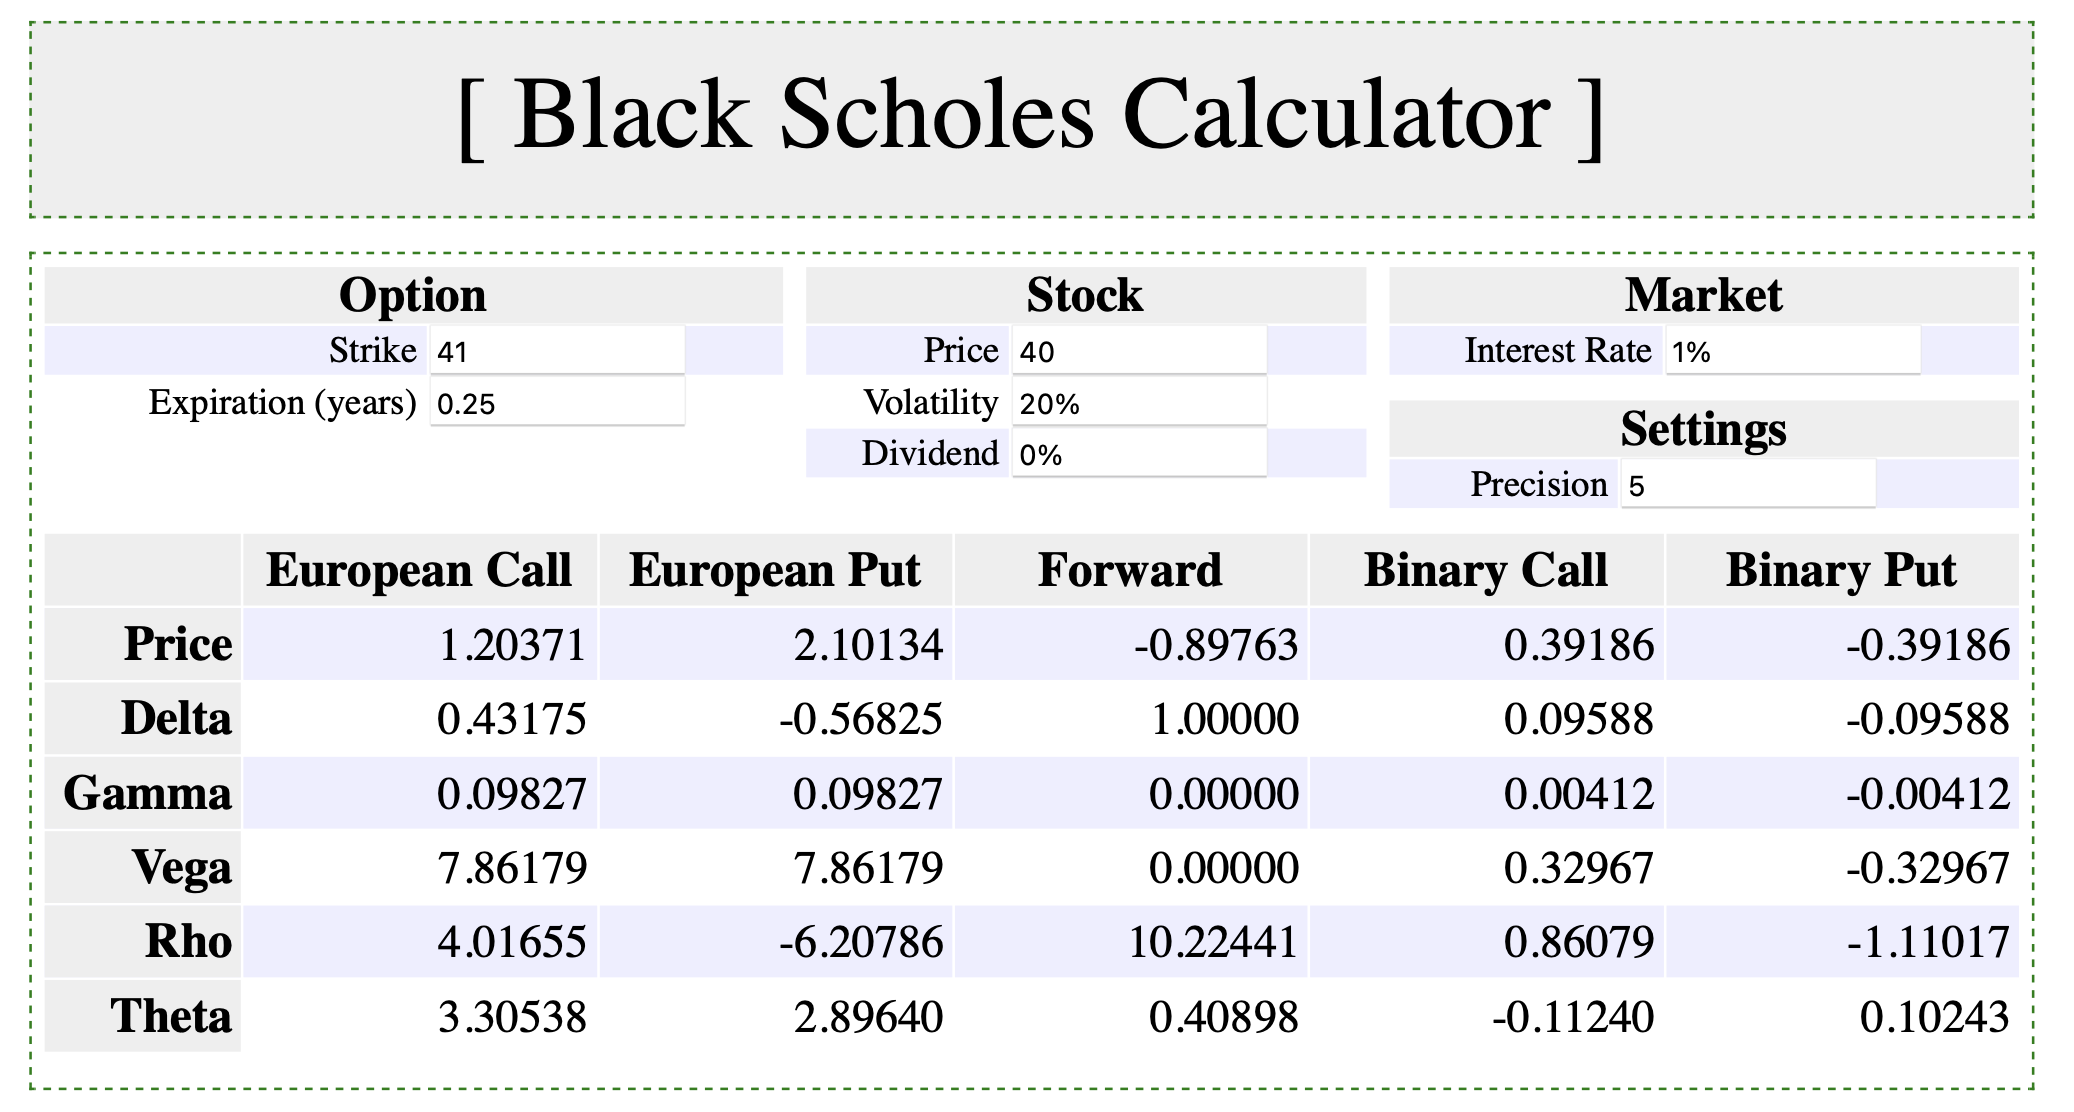
\includegraphics[max width=\textwidth, center]{Q5_2}
		\captionof{figure}{Calculator Results}
		
		This gives the result to be \$ 1.20371.
		
		And I also tried to calculate using Black-Scholes Model, in which the European call option price is calculated as:
		
		$$
		C=S_0e^{-qT}N(d_1)-Ke^{-rT}N(d_2)
		$$
		
		and for we can calculate $d_1=\frac{ln(S_0/K)+(r-q+0.5\sigma^2)T}{\sigma\sqrt{T}}$, and it equals to $\frac{ln(40/41)+(0.01+0.5*0.04)*0.25}{0.2*\sqrt{0.25}}=-0.1719261259$. For $d_2$, we have $d_2=d_1-\sigma \sqrt{T}=d_1-0.1=-0.2719261259$. 
		
		Using the Z-table, we can find that:
		
		\begin{itemize}
			\item $-0.17\rightarrow 0.4325$
			\item $-0.27\rightarrow 0.3936$
		\end{itemize}
		
		Plugging back, we can get $C=S_0*N_{d1}-Ke^{-rT}*N_{d2}=40*0.4325-41*e^{-0.01*0.25}*0.3936=1.202693$. It is roughly \$ 1.2, as the Z-table as not extremely precise. 
		
		\subsection{Part b}
		Calculate $\Delta, \Gamma, \rho$, Vega using formulas for these parameters. Calculate the same parameters approximately using the options calculator.
		
		\textbf{Answers}
		
		As seen from the graph, we have the value of those Greeks to be:
		
		\begin{itemize}
			\item $\Delta=0.43175$
			\item $\Gamma=0.09827$
			\item $\rho=4.01655$
			\item $Vega=7.86179$
			\item $\Theta=3.30538$
			\item $\text{Price}=1.20371$
		\end{itemize}
	
	Because calculating Greeks requires more precision, I can not simply using Z-table, here is a chunk of code for R
	
	\begin{lstlisting}
     # Parameters
     S0 <- 40  # Stock price
     K <- 41   # Strike price
     T <- 0.25  # Time to expiration in years (3 months)
     sigma <- 0.2  # Volatility
     r <- 0.01  # Risk-free rate
     
     # Black-Scholes formula components
     d1 <- (log(S0 / K) + (r + 0.5 * sigma^2) * T) / (sigma * sqrt(T))
     d2 <- d1 - sigma * sqrt(T)
     
     # CDF of d1 and d2 using normal distribution
     N_d1 <- pnorm(d1)
     N_d2 <- pnorm(d2)
     N_prime_d1 <- dnorm(d1)  # PDF of the normal distribution
     
     # Delta
     Delta <- N_d1
     
     # Gamma
     Gamma <- N_prime_d1 / (S0 * sigma * sqrt(T))
     
     # Vega
     Vega <- S0 * sqrt(T) * N_prime_d1
     
     # Theta
     Theta <- -(S0 * N_prime_d1 * sigma) / (2 * sqrt(T)) - r * K * exp(-r * T) * N_d2
     
     # Rho
     Rho <- K * T * exp(-r * T) * N_d2
	\end{lstlisting}

And its printout is: 

\begin{minipage}{\linewidth}
	\begin{Verbatim}
     Delta: 0.4317478 
     Gamma: 0.09827239 
     Vega: 7.861791 
     Theta: -3.305378 
     Rho: 4.01655 
	\end{Verbatim}
\end{minipage}

The same as above.
		
		\subsection{Part c}
		Check that following relationship holds:
		$$
		\Theta+r x \Delta+\frac{1}{2} \sigma^{2} x^{2} \Gamma=r P
		$$
		
		\textbf{Answer}
		
		$\Theta + r \cdot S \cdot \Delta + \frac{1}{2} \sigma^2 \cdot S^2 \cdot \Gamma=-3.30538+0.01\cdot40\cdot0.431748+0.5\cdot0.2^{2}40^{2}\cdot0.098272=0.0120232$, and $rP=0.0120371$.  Those two sides are the same. 
		
		\clearpage
		\section{Question 6}
		What are the parameters affecting prices European and American calls and puts. How do the prices change when one of the parameters changes with all the others remaining the same?
		
		\textbf{Answer}
		
		
		The prices of {European and American} call and put options depend on several factors, including the {underlying asset price}, {strike price}, {time to expiration}, {volatility}, {interest rate}, and {dividends}. Their effects can be seen in the table below (considering parameters to be "higher", to impose effects on prices):
		
	\begin{table}[h]
		\centering
		\begin{tabular}{|l|c|c|}
			\hline
			\textbf{Parameter} & \textbf{Effect on Call Price} & \textbf{Effect on Put Price} \\
			\hline
			\textbf{Underlying Price} ($S$) & Increases ($\uparrow$) & Decreases ($\downarrow$) \\
			\hline
			\textbf{Strike Price} ($K$) & Decreases ($\downarrow$) & Increases ($\uparrow$) \\
			\hline
			\textbf{Time to Expiration} ($T$) & Usually Increases ($\uparrow$) & Usually Increases ($\uparrow$) \\
			\hline
			\textbf{Volatility} ($\sigma$) & Increases ($\uparrow$) & Increases ($\uparrow$) \\
			\hline
			\textbf{Risk-Free Rate} ($r$) & Increases ($\uparrow$) & Decreases ($\downarrow$) \\
			\hline
			\textbf{Dividends} ($D$) & Decreases ($\downarrow$) & Increases ($\uparrow$) \\
			\hline
		\end{tabular}
		\caption{Impact of Various Parameters on Call and Put Prices}
		\label{tab:effects}
	\end{table}
		
		Some explanations:
		
		\begin{enumerate}
		\item Underlying Asset Price ($S$)
		\begin{itemize}
			\item \textbf{Call Options}: Higher $S$ {increases} the call price, as the right to buy at $K$ is more valuable.
			\item \textbf{Put Options}: Higher $S$ {decreases} the put price, as the right to sell at $K$ is less valuable.
		\end{itemize}
		$$
			\frac{\partial C}{\partial S} > 0, \quad \frac{\partial P}{\partial S} < 0
		$$
		
		\item Strike Price ($K$)
		\begin{itemize}
			\item \textbf{Call Options}: Higher $K$ {decreases} the call price.
			\item \textbf{Put Options}: Higher $K$ {increases} the put price.
		\end{itemize}
		$$
			\frac{\partial C}{\partial K} < 0, \quad \frac{\partial P}{\partial K} > 0
		$$
		
		\item Time to Expiration ($T$)
		\begin{itemize}
			\item \textbf{European Options}: Longer $T$ {usually increases} both call and put prices.
			\item \textbf{American Options}: Longer $T$ generally increases option prices, but deep in-the-money puts may behave differently due to early exercise potential.
		\end{itemize}
		$$
			\frac{\partial C}{\partial T} > 0, \quad \frac{\partial P}{\partial T} > 0
		$$
		
	    \item Volatility ($\sigma$)
		\begin{itemize}
			\item Higher \textbf{volatility} {increases} both call and put prices since it increases the probability of large price movements.
		\end{itemize}
		$$
			\frac{\partial C}{\partial \sigma} > 0, \quad \frac{\partial P}{\partial \sigma} > 0
		$$
		
		\item Risk-Free Interest Rate ($r$)
		\begin{itemize}
			\item \textbf{Call Options}: Higher $r$ {increases} call prices because the present value of $K$ decreases.
			\item \textbf{Put Options}: Higher $r$ {decreases} put prices for the same reason.
		\end{itemize}
	    $$
			\frac{\partial C}{\partial r} > 0, \quad \frac{\partial P}{\partial r} < 0
		$$
		
		\item Dividends ($D$)
		\begin{itemize}
			\item \textbf{Call Options}: Higher dividends {reduce} call prices since they lower $S$.
			\item \textbf{Put Options}: Higher dividends {increase} put prices as $S$ declines.
		\end{itemize}
	    $$
			\frac{\partial C}{\partial D} < 0, \quad \frac{\partial P}{\partial D} > 0
		$$
		\end{enumerate}
		
		
		
		\clearpage
		\section{Question 7}
		Suppose that we have three European calls with strikes 60, 65, and 70 and the same maturity 1 month. Their prices are $9.00$, $7.00$, $4.00$. Is it possible to do an arbitrage?
		
		\textbf{Answer}
		
		To determine if there is an arbitrage opportunity, we need to check whether the given call option prices satisfy the conditions of a butterfly spread, ensuring that no arbitrage violation occurs.

		For European call options with the same expiry, the call option prices must be non-increasing in strike prices:
		
		\[
		C(K_1) \geq C(K_2) \geq C(K_3)
		\]
		
		Given prices:
		
		\[
		C(60) = 9.00, \quad C(65) = 7.00, \quad C(70) = 4.00
		\]
		
		This satisfies the basic monotonicity condition:
		
		\[
		9.00 \geq 7.00 \geq 4.00
		\]
		
		Thus, there is no immediate arbitrage due to mis-pricing of monotonicity.
		
		A butterfly spread using these strikes consists of:
		
		\begin{itemize}
			\item Long 1 Call at \( K_1 = 60 \)
			\item Short 2 Calls at \( K_2 = 65 \)
			\item Long 1 Call at \( K_3 = 70 \)
		\end{itemize}
		
		The cost of setting up the butterfly spread is $C(60) - 2C(65) + C(70)$, thus substituting the given prices $9.00 - 2(7.00) + 4.00 = 9.00 - 14.00 + 4.00 = -1.00$
		
		Since the total cost of the butterfly spread is negative, it means that an arbitrage opportunity exists. We are receiving $1.00$ upfront while ensuring a non-negative payoff at expiration.
		
		To exploit this arbitrage, we should:
		
			\begin{itemize}
			\item Buy 1 Call at \( K_1 = 60 \) for $9.00$.
			\item Sell 2 Calls at \( K_2 = 65 \) for $7.00$ each (receive $14.00$).
			\item Buy 1 Call at \( K_3 = 70 \) for $4.00$.
		\end{itemize}
		
		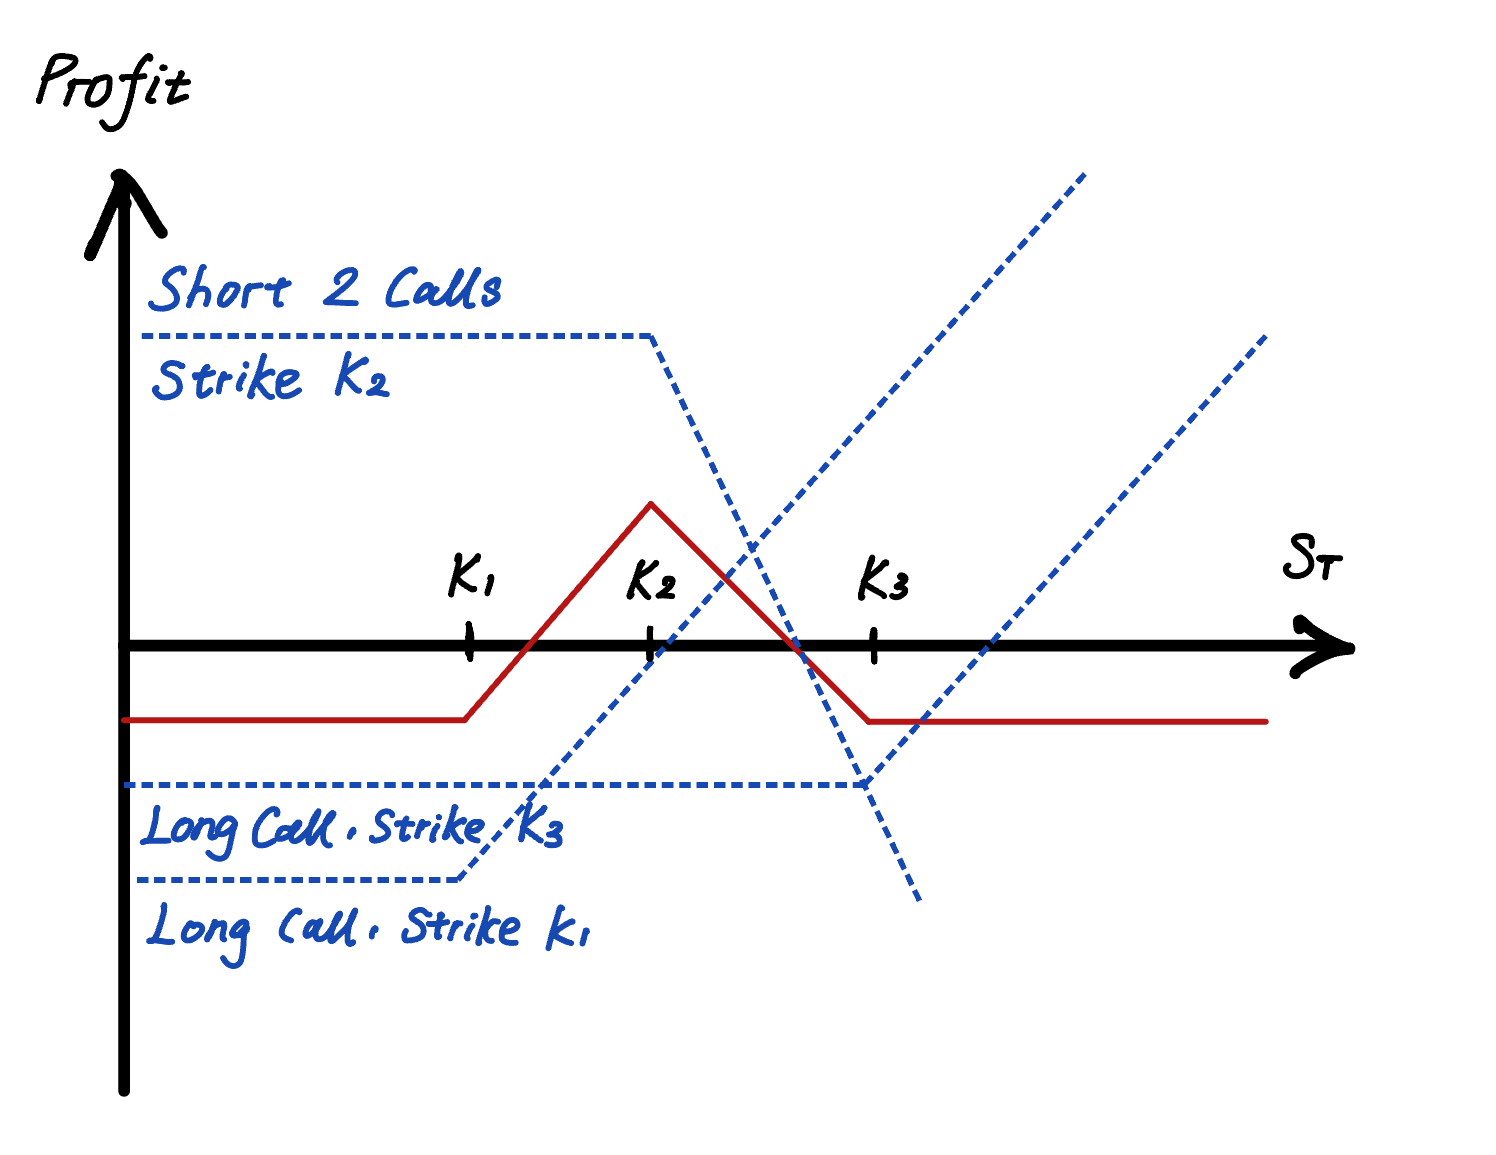
\includegraphics[max width=0.6\textwidth, center]{Q7}
		\captionof{figure}{Butterfly Spread Using Call Option}
		
		Total cost = -$1.00$.
		
		At expiration, the payoff of the butterfly spread is always non-negative, so this setup guarantees a risk-free profit.
		
		There exists an arbitrage opportunity exists because the cost of the butterfly spread is negative, and we can execute this arbitrage to receive $1.00$ upfront with no risk.
		
		\clearpage
		\section{Question 8}

		Suppose that current stock price is $\$50$. Its annualized volatility is $30 \%$ and annualized return $10 \%$ i.e. we assume that the stock price follows ${d} {X}_{{t}}=0.1 {X}_{{t}} {dt}+0.3 {X_t} {dW}$. Write the probability density function for the stock in 1 year. What is the mean and standard deviation of the terminal stock price? (standard deviation of price, not of return)
		
		\textbf{Answer}
		
		(This number is not doubtful)
			
			The stock price \( X_1 \) at time \( t = 1 \) follows a log-normal distribution:
			
			\[
			f(x) = \frac{1}{x \sigma \sqrt{2 \pi}\sqrt{t}} \exp\left( -\frac{\left( \ln(x) -ln(X_0)- \left( \mu - \frac{1}{2} \sigma^2 \right)t \right)^2}{2 \sigma^2} \right)
			\]
			
			Here:
			\begin{itemize}
				\item \( \mu = 0.1 \) is the drift (annualized return),
				\item \( \sigma = 0.3 \) is the volatility (annualized standard deviation of return),
				\item \( x \) is the value of the stock price \( X_1 \) at time \( t = 1 \).
			\end{itemize}
			
			Thus, the PDF for \( X_1 \) becomes:
			
			\[
			f(x) = \frac{1}{x (0.3) \sqrt{2 \pi}} \exp\left( -\frac{(\ln(x) -3.967023005)^2}{2 (0.3)^2} \right)
			\]
			
			We can get that the \underline{mean} of \( X_1 \) is $\mathbb{E}[X_0] = X_0 e^{( \mu t )}$, and substituting the given values $	\mathbb{E}[X_0] = 50e^{( 0.1 * t)} = 50 e^{0.1}$. Using \(e^{0.1} \approx 1.10517 \), we get $\mathbb{E}[X_0] \approx 50 \times 1.10517 = 55.2585$. 
			
			The \underline{variance} of \( X_0\) is $
			\text{SD}(X_0) = X_0^2 \exp( 2\mu t)*(\exp(\sigma^2t)-1)$, and substituting the values we have $Var(X_1)=50^2*e^{2*0.1*t}(e^{0.09}-1)=287.5618$. Then take its square, we can get 16.9576.
			
			
			\begin{itemize}
				\item The \underline{mean} of the terminal stock price is approximately \( \mathbb{E}[X_1] \approx 55.2585\).
				\item The \underline{standard deviation} of the terminal stock price is approximately \( \text{SD}(X_1) \approx 16.9576\).
			\end{itemize}
			
		
		
		
		
		
	\end{document}